\section{Supplemental Figures}

\begin{figure}[h]
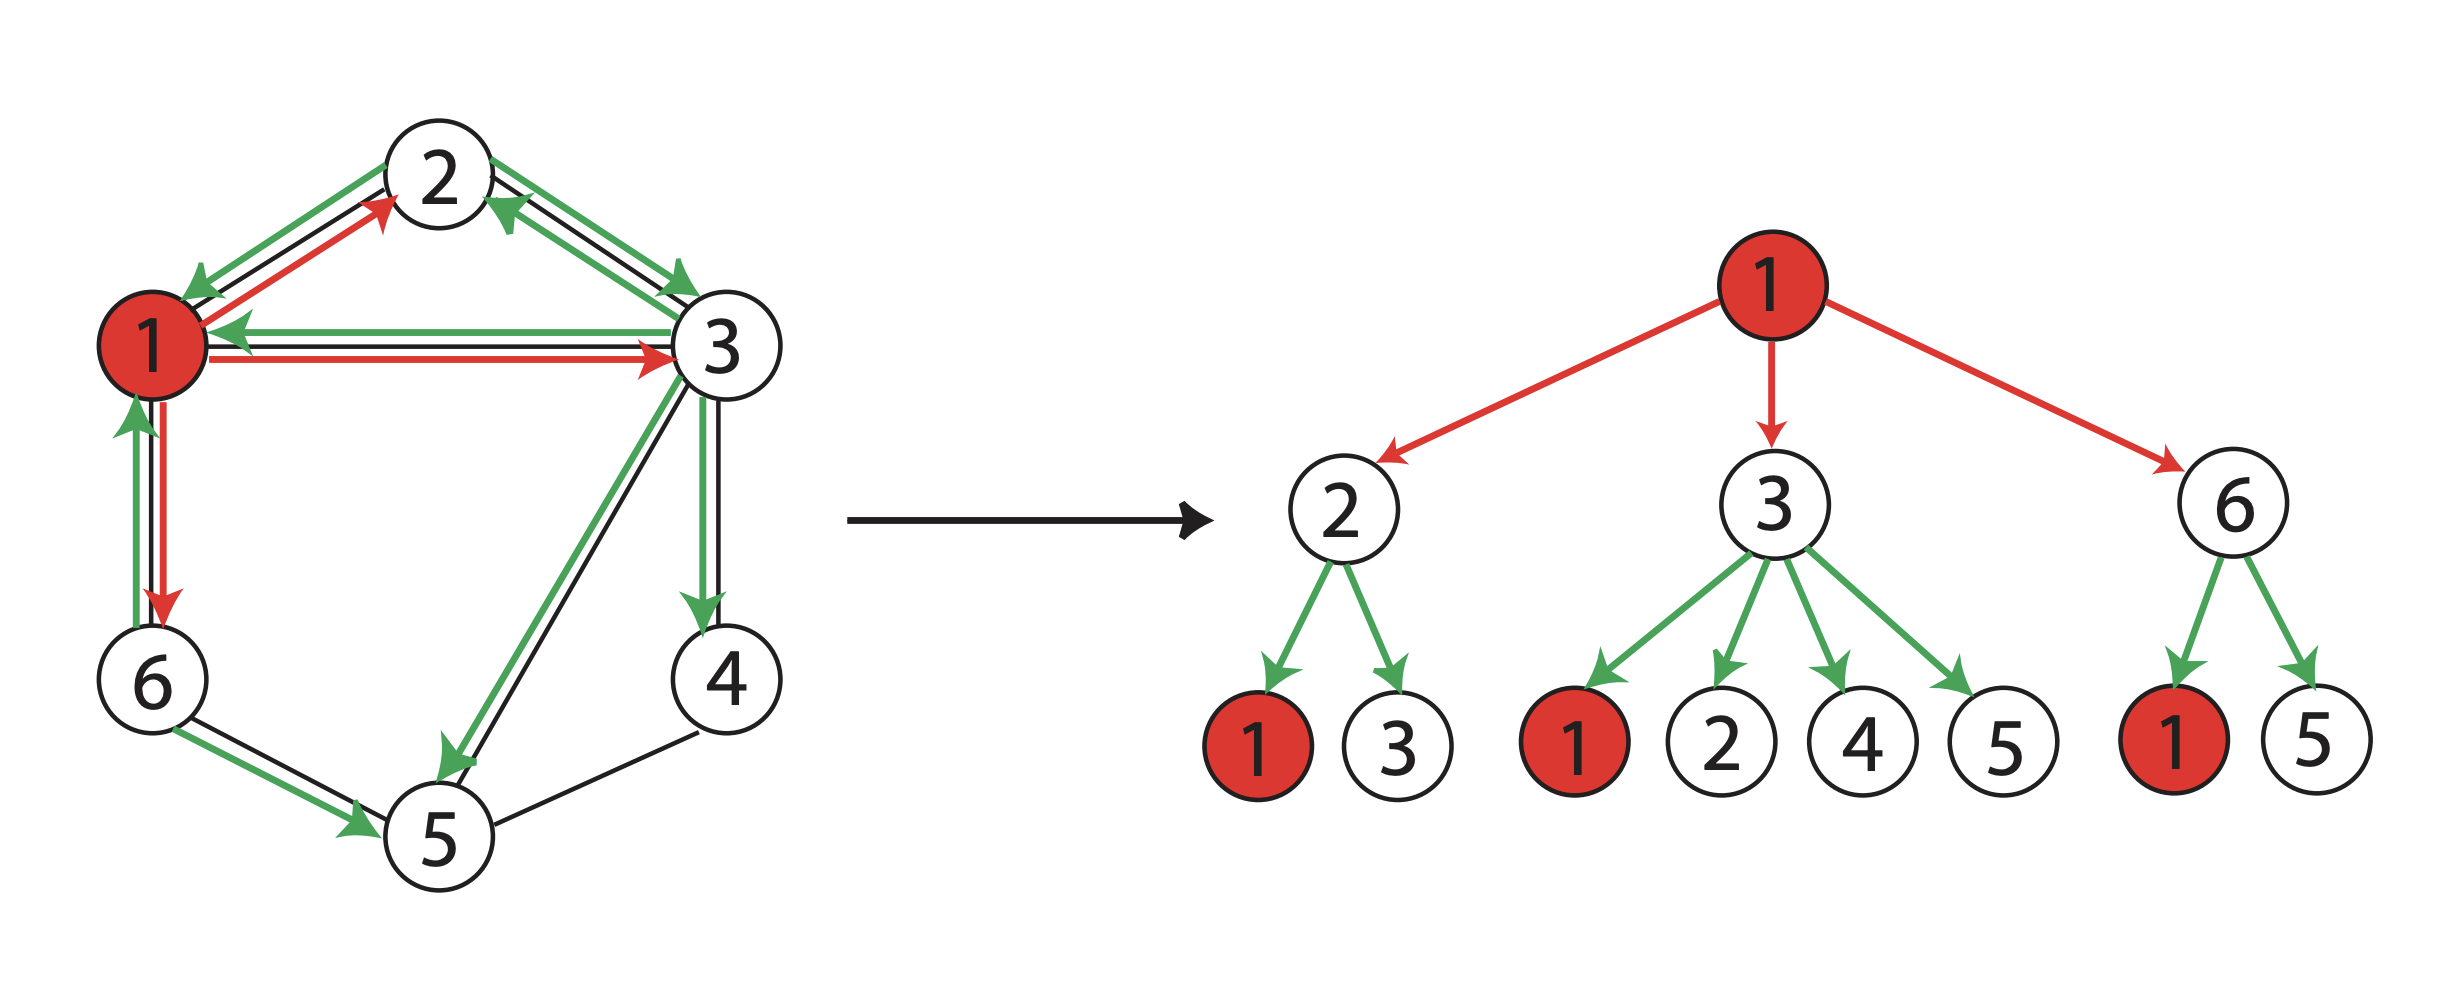
\includegraphics[width=\textwidth]{figs/tree_height_2.png}
\caption{Schematic showing the nodes reachable within two hops of the root node 1. Figure taken from \citet{SchweitzerPASCAL2011}.}
\label{fig:tree}
\end{figure}

\begin{figure}[h]
\centering
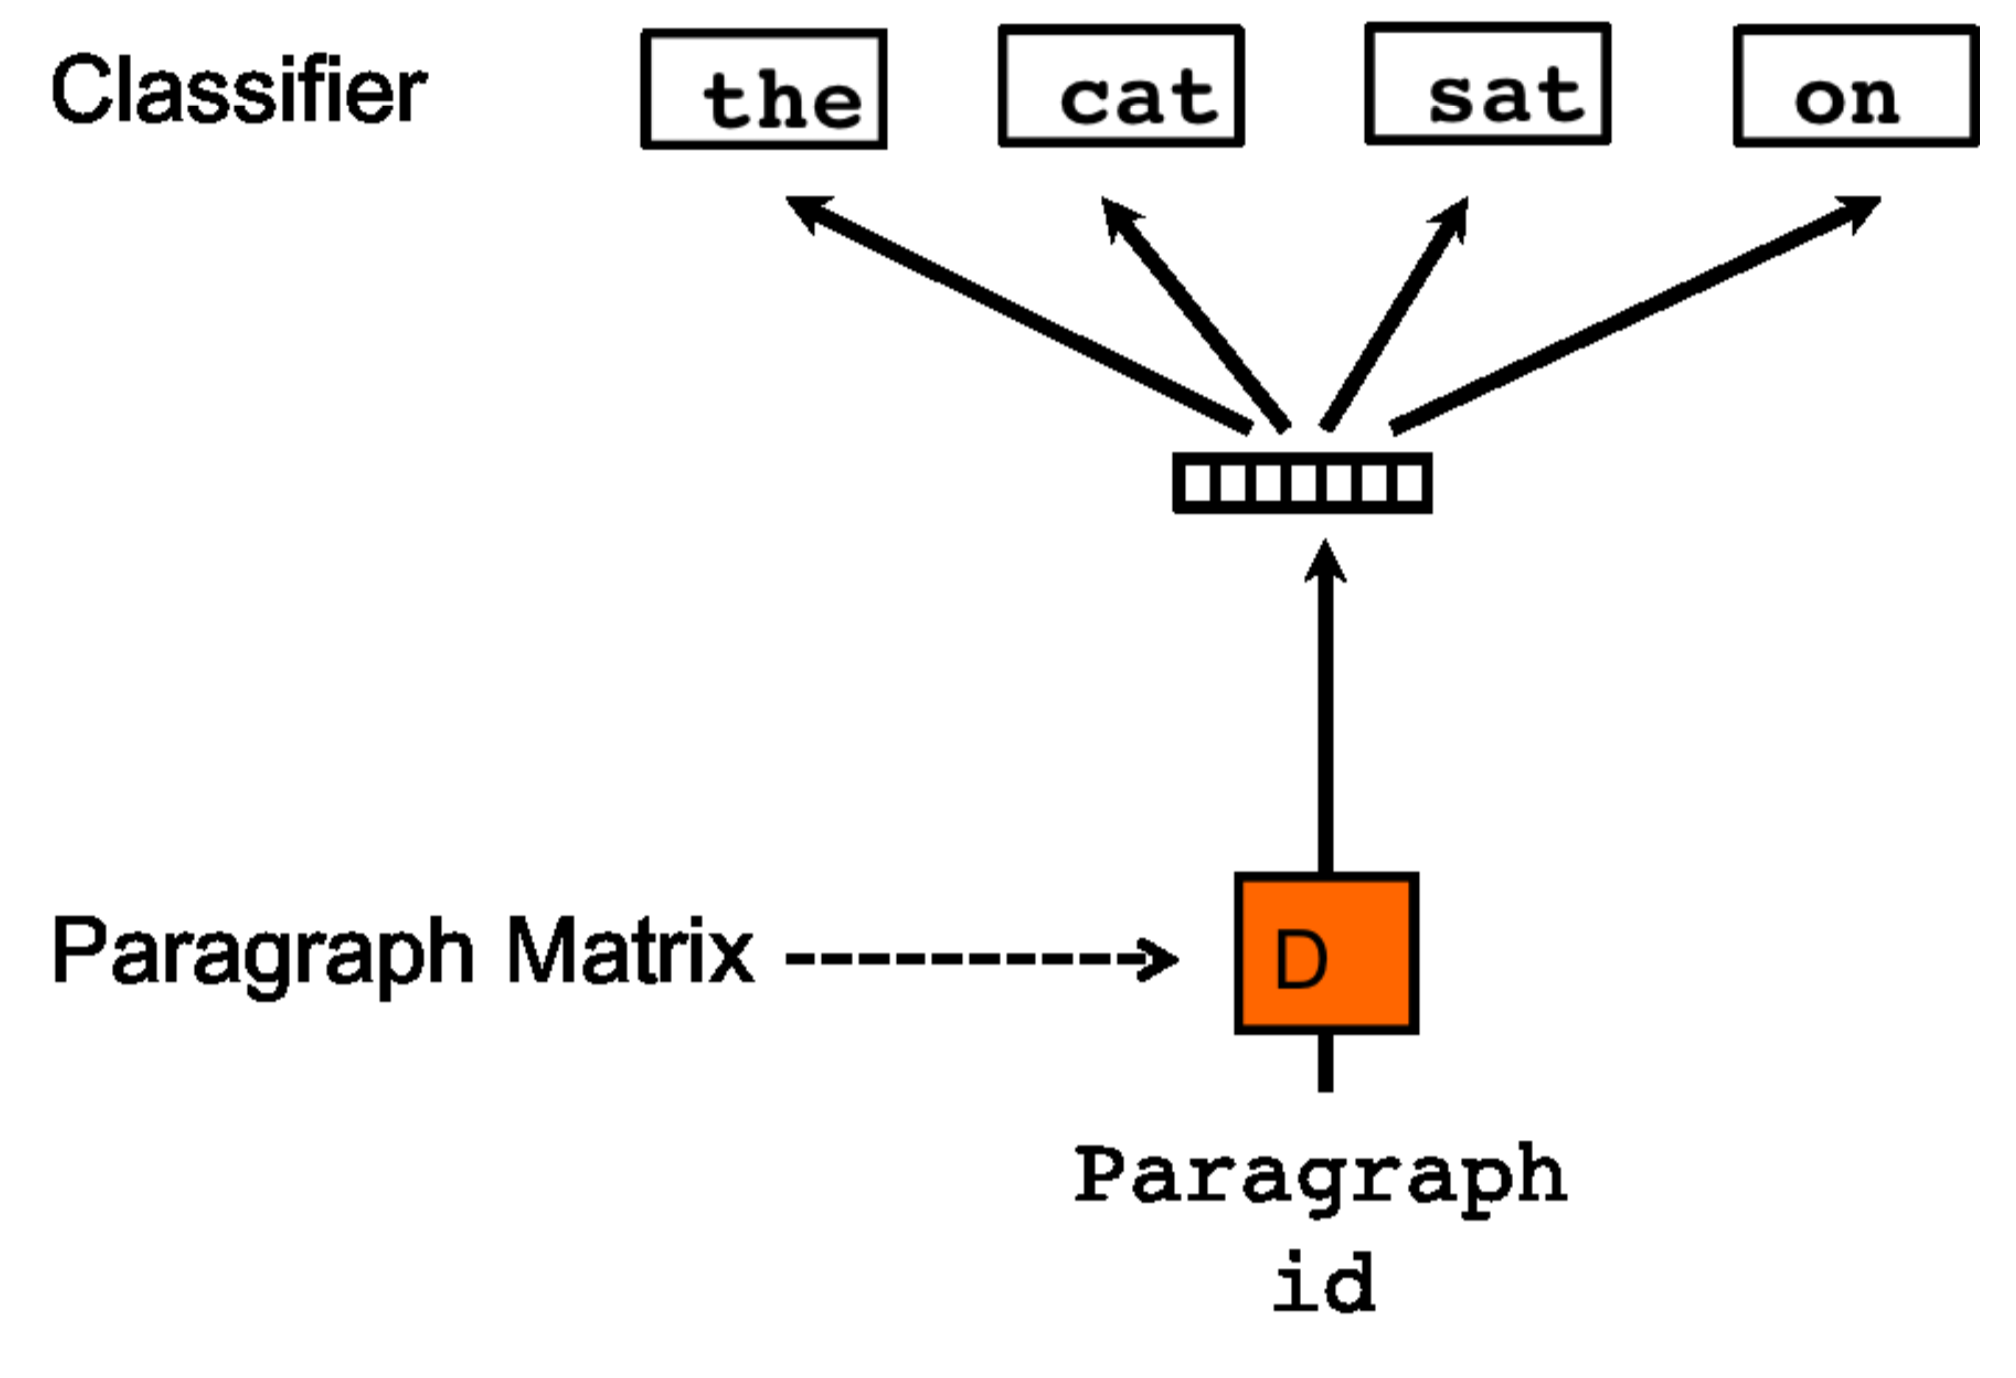
\includegraphics[width=0.6\textwidth]{figs/paragraph2vec.png}
\caption{Schematic of \textit{doc2vec} prediction taken from \citet{Le2014}. The document vector is used to predict words in a small window.}
\label{doc2vec}
\end{figure}

% histograms
\begin{figure}
\centering
\begin{subfigure}{0.45\linewidth}
    \includegraphics[width=\linewidth]{../plots/pass_plots/deg_4_dims_128_epochs_100/E_LOGP_histogram.png}
    \caption{logP}
\end{subfigure}
\begin{subfigure}{0.45\linewidth}
    \includegraphics[width=\linewidth]{../plots/pass_plots/deg_4_dims_128_epochs_100/E_WEIGHT_histogram.png}
    \caption{Weight}
\end{subfigure}
\caption{Histograms for predicted compound properties. These exhibit a heavy right skew.}
\label{fig:histograms}
\end{figure}

\begin{figure}[h]
\begin{subfigure}{0.45\textwidth}
\centering
\includegraphics[width=\textwidth]{../plots/pass_plots/deg_3_dims_256_epochs_10/is_div5.png}
\caption{10 epochs}
\label{fig:isdiv5deg_3_dims_256_epochs_10}
\end{subfigure}
\begin{subfigure}{0.45\textwidth}
\includegraphics[width=\textwidth]{../plots/pass_plots/deg_3_dims_256_epochs_100/is_div5.png}
\caption{100 epochs}
\label{fig:isdiv5deg_3_dims_256_epochs_100}
\end{subfigure}
\caption{256-dimensional embedding for degree 3 subtrees, visualized in 2 dimensions via UMAP. Diversity V Set compounds colored in orange, while other Open Set compounds colored in blue. The diversity compounds are spread well throughout the embedding space.}
\end{figure}

\begin{figure}[h]
\begin{subfigure}{0.45\textwidth}
\centering
\includegraphics[width=\textwidth]{../plots/pass_plots/deg_4_dims_128_epochs_10/is_div5.png}
\caption{10 epochs}
\label{fig:deg4_10_isdiv5}
\end{subfigure}
\begin{subfigure}{0.45\textwidth}
\includegraphics[width=\textwidth]{../plots/pass_plots/deg_4_dims_128_epochs_100/is_div5.png}
\caption{100 epochs}
\label{fig:deg4isdiv5}
\end{subfigure}
\caption{128-dimensional embedding for degree 4 subtrees, visualized in 2 dimensions via UMAP. Diversity V Set compounds colored in orange, while other Open Set compounds colored in blue. The diversity compounds are spread well throughout the embedding space.}
\end{figure}

%%%%%%%%%%%%%%%%%%%%%%%%

\begin{figure*}
\centering

\begin{subfigure}{0.45\textwidth}
    \includegraphics[width=\linewidth]{../plots/pass_plots/deg_3_dims_256_epochs_10/E_LOGP.png}
    \caption{logP}
\end{subfigure}
\begin{subfigure}{0.45\textwidth}
    \includegraphics[width=\linewidth]{../plots/pass_plots/deg_3_dims_256_epochs_10/E_WEIGHT.png}
    \caption{Weight}
\end{subfigure}
\begin{subfigure}{0.45\textwidth}
    \includegraphics[width=\linewidth]{../plots/pass_plots/deg_3_dims_256_epochs_10/Predicted_Activity_Antiinflammatory.png}
    \caption{Antiinflammatory}
\end{subfigure}
\begin{subfigure}{0.45\textwidth}
    \includegraphics[width=\linewidth]{../plots/pass_plots/deg_3_dims_256_epochs_10/Predicted_Activity_Carcinogenic.png}
    \caption{Carcinogenic}
\end{subfigure}
\begin{subfigure}{0.45\textwidth}
    \includegraphics[width=\linewidth]{../plots/pass_plots/deg_3_dims_256_epochs_10/Predicted_Activity_Immunostimulant.png}
    \caption{Immunostimulant}
\end{subfigure}
\begin{subfigure}{0.45\textwidth}
    \includegraphics[width=\linewidth]{../plots/pass_plots/deg_3_dims_256_epochs_10/Predicted_Activity_Immunosuppressant.png}
    \caption{Immunosuppressant}
\end{subfigure}
\caption{256-dimensional embedding for degree 3 subtrees trained for 10 epochs}
\label{fig:deg_3_dims_256_epochs_10}
\end{figure*}

%%%%%%%%%%%%%%%%%%%%%%%%%%%%

\begin{figure*}
\centering

\begin{subfigure}{0.45\textwidth}
    \includegraphics[width=\linewidth]{../plots/pass_plots/deg_3_dims_256_epochs_100/E_LOGP.png}
    \caption{logP}
\end{subfigure}
\begin{subfigure}{0.45\textwidth}
    \includegraphics[width=\linewidth]{../plots/pass_plots/deg_3_dims_256_epochs_100/E_WEIGHT.png}
    \caption{Weight}
\end{subfigure}
\begin{subfigure}{0.45\textwidth}
    \includegraphics[width=\linewidth]{../plots/pass_plots/deg_3_dims_256_epochs_100/Predicted_Activity_Antiinflammatory.png}
    \caption{Antiinflammatory}
\end{subfigure}
\begin{subfigure}{0.45\textwidth}
    \includegraphics[width=\linewidth]{../plots/pass_plots/deg_3_dims_256_epochs_100/Predicted_Activity_Carcinogenic.png}
    \caption{Carcinogenic}
\end{subfigure}
\begin{subfigure}{0.45\textwidth}
    \includegraphics[width=\linewidth]{../plots/pass_plots/deg_3_dims_256_epochs_100/Predicted_Activity_Immunostimulant.png}
    \caption{Immunostimulant}
\end{subfigure}
\begin{subfigure}{0.45\textwidth}
    \includegraphics[width=\linewidth]{../plots/pass_plots/deg_3_dims_256_epochs_100/Predicted_Activity_Immunosuppressant.png}
    \caption{Immunosuppressant}
\end{subfigure}
\caption{256-dimensional embedding for degree 3 subtrees trained for 100 epochs.}
\label{fig:deg_3_dims_256_epochs_100}
\end{figure*}

%%%%%%%%%%%%%%%%%%%%

\begin{figure*}
\centering

\begin{subfigure}{0.45\textwidth}
    \includegraphics[width=\linewidth]{../plots/pass_plots/deg_4_dims_128_epochs_10/E_LOGP.png}
    \caption{logP}
\end{subfigure}
\begin{subfigure}{0.45\textwidth}
    \includegraphics[width=\linewidth]{../plots/pass_plots/deg_4_dims_128_epochs_10/E_WEIGHT.png}
    \caption{Weight}
\end{subfigure}
\begin{subfigure}{0.45\textwidth}
    \includegraphics[width=\linewidth]{../plots/pass_plots/deg_4_dims_128_epochs_10/Predicted_Activity_Antiinflammatory.png}
    \caption{Antiinflammatory}
\end{subfigure}
\begin{subfigure}{0.45\textwidth}
    \includegraphics[width=\linewidth]{../plots/pass_plots/deg_4_dims_128_epochs_10/Predicted_Activity_Carcinogenic.png}
    \caption{Carcinogenic}
\end{subfigure}
\begin{subfigure}{0.45\textwidth}
    \includegraphics[width=\linewidth]{../plots/pass_plots/deg_4_dims_128_epochs_10/Predicted_Activity_Immunostimulant.png}
    \caption{Immunostimulant}
\end{subfigure}
\begin{subfigure}{0.45\textwidth}
    \includegraphics[width=\linewidth]{../plots/pass_plots/deg_4_dims_128_epochs_10/Predicted_Activity_Immunosuppressant.png}
    \caption{Immunosuppressant}
\end{subfigure}
\caption{128-dimensional embedding for degree 4 subtrees trained for 10 epochs.}
\label{fig:deg_4_dims_128_epochs_10}
\end{figure*}

%%%%%%%%%%%%%%%%%%%%%%%%%%%%%%%%%%%%

\begin{figure*}
\centering

\begin{subfigure}{0.45\textwidth}
    \includegraphics[width=\linewidth]{../plots/pass_plots/deg_4_dims_128_epochs_100/E_LOGP.png}
    \caption{logP}
\end{subfigure}
\begin{subfigure}{0.45\textwidth}
    \includegraphics[width=\linewidth]{../plots/pass_plots/deg_4_dims_128_epochs_100/E_WEIGHT.png}
    \caption{Weight}
\end{subfigure}
\begin{subfigure}{0.45\textwidth}
    \includegraphics[width=\linewidth]{../plots/pass_plots/deg_4_dims_128_epochs_100/Predicted_Activity_Antiinflammatory.png}
    \caption{Antiinflammatory}
\end{subfigure}
\begin{subfigure}{0.45\textwidth}
    \includegraphics[width=\linewidth]{../plots/pass_plots/deg_4_dims_128_epochs_100/Predicted_Activity_Carcinogenic.png}
    \caption{Carcinogenic}
\end{subfigure}
\begin{subfigure}{0.45\textwidth}
    \includegraphics[width=\linewidth]{../plots/pass_plots/deg_4_dims_128_epochs_100/Predicted_Activity_Immunostimulant.png}
    \caption{Immunostimulant}
\end{subfigure}
\begin{subfigure}{0.45\textwidth}
    \includegraphics[width=\linewidth]{../plots/pass_plots/deg_4_dims_128_epochs_100/Predicted_Activity_Immunosuppressant.png}
    \caption{Immunosuppressant}
\end{subfigure}
\caption{128-dimensional embedding for degree 4 subtrees trained for 100 epochs.}
\label{fig:deg_4_dims_128_epochs_100}
\end{figure*}

